\newpage
\section{Order}
Orders are a new feature in \salespoint. The intention was to prepare the old databaskets for development of web applications and extend them to collaborate with our new inventory, providing the opportunity of individual pricing and final payment.

\begin{figure}[ht]
	\centering
  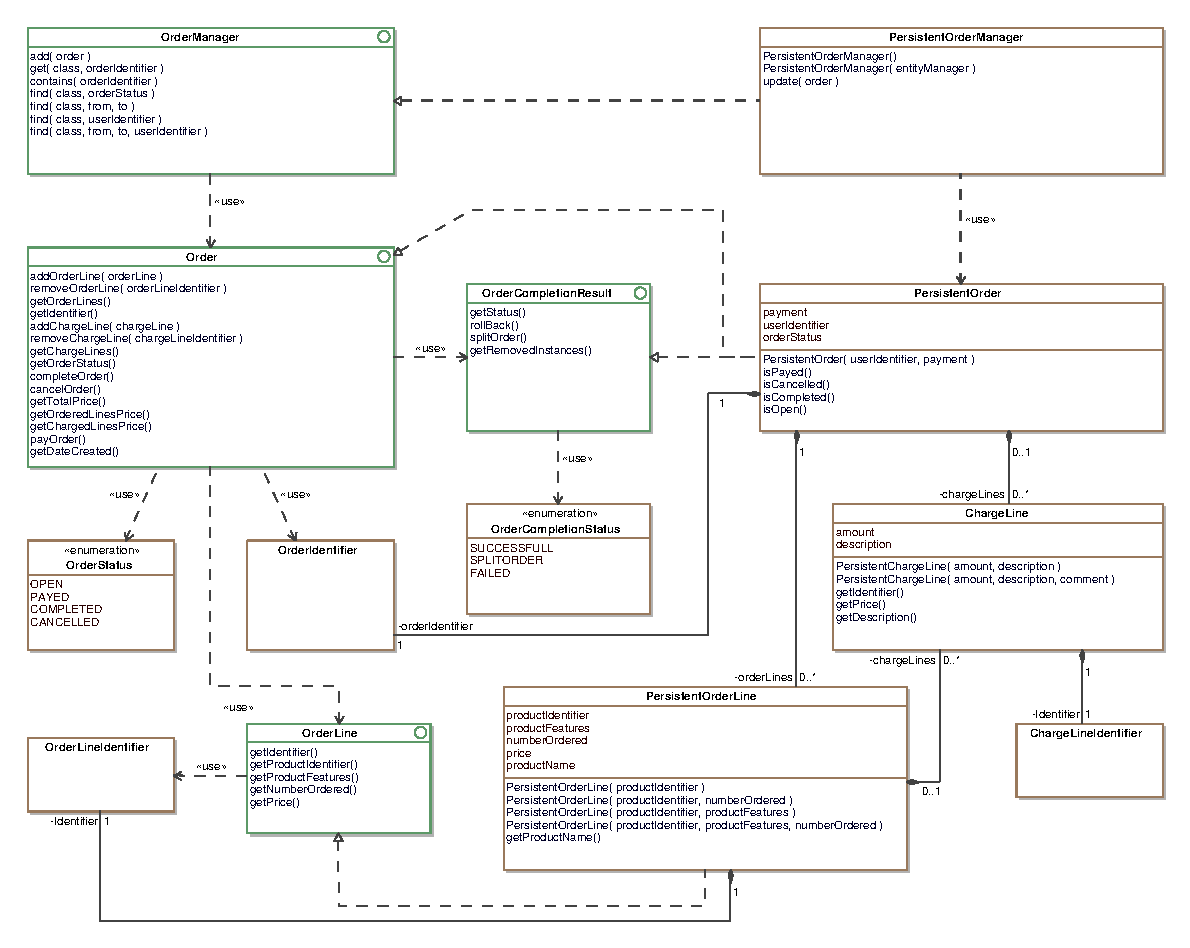
\includegraphics[width=1.0\textwidth]{images/Order_Overview.eps}
	\label{order_overview}
	\caption{Order - Class Overview}
\end{figure}

\subsection{\code{Order} - The main data structure}
We created the \code{Order} as main data structure to access the functionality above. An \code{Order} can be imagined as sheet of paper which basically consists of lines representing the ordered products (\code{OrderLine}) and lines that are not bound to a concrete product but which cause charge (\code{ChargeLine}).

\code{ChargeLines} make it possible to add individual charge to orders. For example they can be used to define forwarding charges or other special charges produced by this order.

To identify the actor of this order the \code{UserIdentifier} from orderer is also be needed. The \code{SalesChannel} should be used to save information from which channel the order was created (e.g. telephone, internet or mail).

\code{Orders} are lifecycle-objects. The lifecycle covers four states which are defined by enumeration type \code{OrderEntryStatus}. After all the lifecycle has restrictions in changing states, which are transposed automatic by the according methods. \code{COMPLETED} is one of the final states and it's not possible to change the state of such \code{Orders}. The figure \ref{order_statemachine} shows a state machine which illustrates the lifecycle of \code{Orders}.

\begin{figure}[ht]
	\centering
  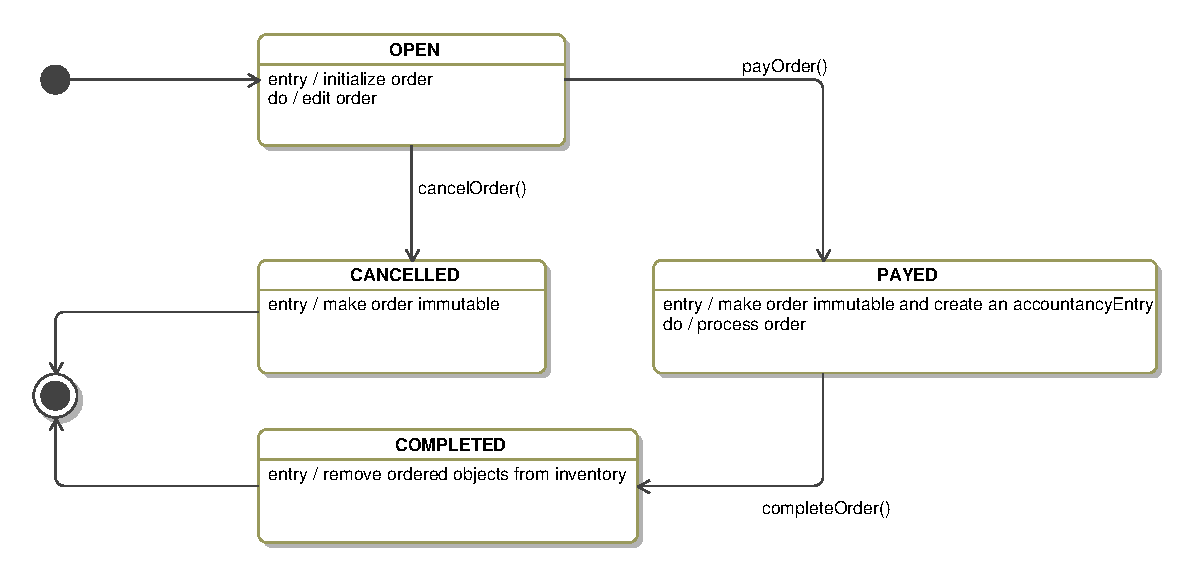
\includegraphics[width=1.0\textwidth]{images/Order_StateMachine.eps}
  \label{order_statemachine}
	\caption{Order - Lifecycle}
\end{figure}  

As you can see an OrderEntry can only completely modified in state \code{OPEN}. \code{PAYED}, \code{CANCELLED} and \code{COMPLETED} \code{Orders} are immutable!  Calling the \code{payOrder()} method changes the state and calls the accountancy to create a \code{PaymentEntry}. Ordered objects will be removed from inventory not until the \code{completeOrder()} method is called.  

\subsection{\code{OrderLine} - Representing ordered objects}
\code{OrderLines} containing all information needed to identify product instances and deal with them. Every \code{OrderLine} represents one ordered \code{Product} that contains data about its \code{ProductType} and \code{ProductFeatures}. 

Every \code{OrderLine} is identified by one unique \code{OrderLineIdentifier}. Hence an \code{Order} contains an \code{OrderLine} for every ordered product. 

As well as \code{Orders}, \code{OrderLines} can also contain \code{ChargeLines} that can be used to deploy discounts or bonuses. The \code{PersistentOrderLine} class is a basic implementation of \code{OrderLine} interface and will be sufficient at most use cases.

\subsection{\code{ChargeLine} - Representing additional charge}
\code{ChargeLines} representing additional charge for \code{OrderLines} and \code{OrderEntrys}. 

Every \code{ChargeLine} is identified by one unique \code{ChargeLineIdentifier}. They can have a description and a comment. The amount of ChargeLines will be involved in price calculation of \code{Orders} and \code{OrderLines}.

\subsection{\code{OrderCompletionResults} - Cases of completed \code{Orders}}
As per description in chapters before the \code{completeOrder()} method will remove the product instances from \code{Inventory}. But what will happen if these instances are no more present in the inventory because they are removed by other transactions? As you can see it is a little bit more complicated. 

Therefore we provide \code{OrderCompletionResult} interface. The \code{OrderCompletionResult} will be returned from the \code{completeOrder()} method and has three possible results:

\begin{itemize}
\item \code{SUCCESSFULL}: This result will only be returned if all product instances we successfully removed from \code{Inventory} and the \code{Order} is truly completed. 
\item \code{SPLIT}: If not all product instances were found in the \code{Inventory} the order will be splitted into two \code{Orders}. One complete \code{Order}, that contains all product instances that are removed successfully from \code{Inventory} and one \code{Order} in \code{PAYED} state, which contains all product instances that could not be removed from \code{Inventory}. The uncompleted is contained in the returned \code{OrderCompletionResult} with \code{SPLIT} state.
\item \code{FAILED}: If the \code{completeOrder()} method fails, an \code{OrderCompletionResult} in \code{FAILED} state will be returned. This can happen if the \code{completeOrder()} method is used with \code{Orders} that are not in \code{PAYED} state for example.
\end{itemize}

\subsection{\code{OrderManager} - The interface to JPA}
To simplify the management of \code{Orders} we have created the \code{PersistentOrderManager} which implements the \code{OrderManager} interface. 

With that manager class you can persist, update, find and remove \code{Orders}. Contained objects like \code{OrderLines} and \code{ChargeLines} will also be persisted, updated or removed with the\code{Order} they depend on (Cascade).

\code{PersistentOrderManager} is a non-Entity class and cannot be persisted! The Manager will be initialized from the \code{Shop} class and can also be requested from there.

